% Suggested insertion point:
% Place this fragment at the end of the Simulation Design section, after the
% paragraph on recorded metrics and tail fitting, and immediately before
% \section{Results}.

\paragraph{Representative-state and extension design.}
In addition to the replication benchmark, we generated representative
graph-and-accessibility galleries for the validated headline scenarios and ran
a focused extension suite for planarity and accessibility semantics. The
headline representative galleries were drawn from the validated medium-scale
replication bundle by selecting, for each headline scenario, the replication
whose summary statistics were closest to the scenario mean over maximum degree,
degree Gini, clustering, and mean edge length. We then reran those selected
parameter-seed combinations and computed node-level gravity accessibility on the
realized graph so that the graph morphology and induced accessibility field
could be shown together on a common color scale.

The focused extension suite was designed as a two-stage isolation exercise for
transport-oriented mechanism families beyond the baseline generalized model. It
used $N=220$ final nodes and four replications per scenario. In the first
stage, we isolated \emph{planarity handling}: we held the arrival process,
capacity, and cost environment fixed, then varied only the crossing rule across
three matched free-geometry cases---\texttt{none},
\texttt{reject\_crossings}, and \texttt{split\_crossings}. These runs used
uniform arrivals, no lattice framing, weak cost pressure ($\phi=0$), high
capacity ($K=64$), and $\kappa=4$, so the observed differences can be
interpreted as the effect of the planarity rule itself.

In the second stage, we isolated \emph{accessibility semantics within an active
planar transport-growth setting}. Here the geometry and split-capable growth
environment were held fixed using a square-lattice design with frontier-based
arrivals, queen adjacency, a wide local candidate set, high capacity, and weak
cost pressure. Within that shared setting, we compared four cases: a
reject-planarity control with no access weighting, split planarity with
target-only network access, split planarity with seed-based arrival and target
access, and split planarity with opportunity-based arrival and target access.
Across both stages we recorded admitted crossing candidates, split events,
generated intersection nodes, graph morphology, and realized accessibility
fields. Figure~\ref{fig:extension-design-schematic} summarizes this logic:
Panel A varies only the planarity rule, while Panel B varies only the
accessibility semantics within a split-capable planar regime.

\begin{figure}[htbp]
\centering
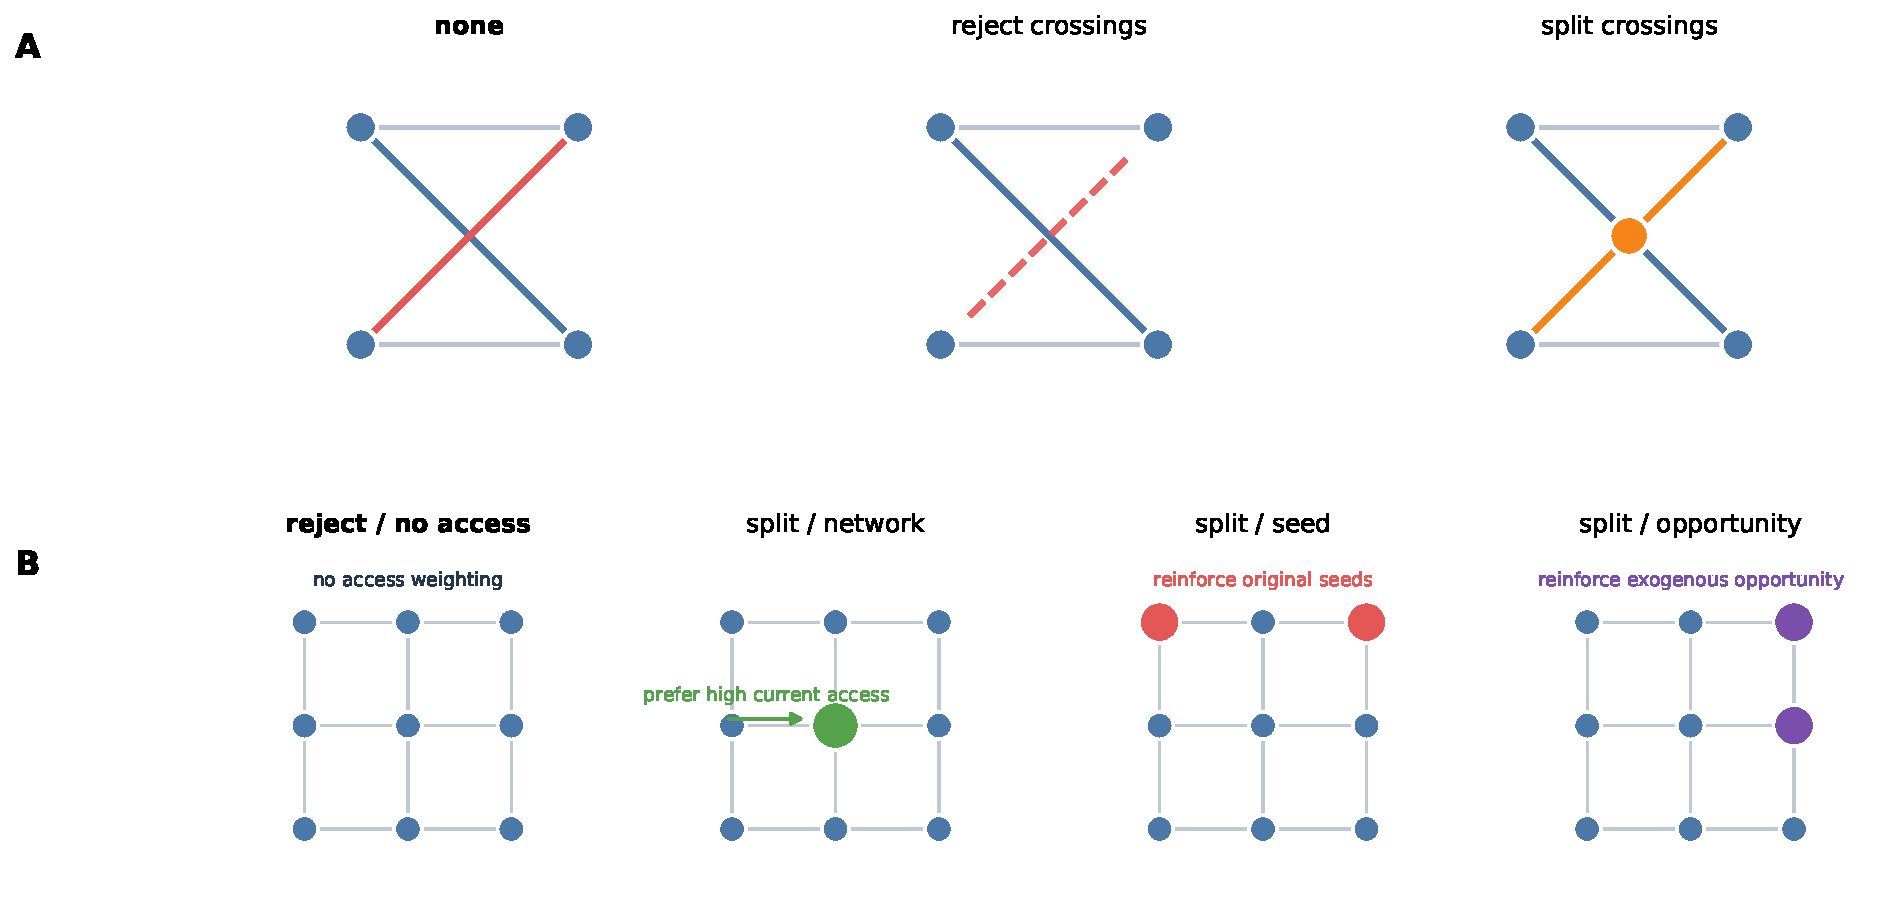
\includegraphics[width=0.98\textwidth]{../results/beyond_paper_focused_20260422_medium/figures/figure_extension_design_schematic.pdf}
\caption{Stylized design logic of the focused extension suite. Panel A isolates
planarity handling by holding the free-geometry growth environment fixed and
varying only whether crossings are retained, rejected, or split into new
junctions. Panel B isolates accessibility semantics by holding the
split-capable planar environment fixed and varying only the destination logic:
no access weighting, network access, seed-based access, or opportunity-based
access.}
\label{fig:extension-design-schematic}
\end{figure}
